\section{问题重述}
\subsection{问题背景}
塔式太阳能光热发电作为一种低碳环保的清洁能源技术,其对我国``可持续发展''战略有着重大意义。
定日镜是一种由平板反射镜、镜架、跟踪传动机构机器控制系统等组成的聚光装置。发电站中心塔周围分布着上千个定日镜,称为镜场,镜场之中的定日镜数量庞大,于是开发定日镜镜场的光学效率的计算和优化成为了重要课题。

\begin{figure}[H]
\centering
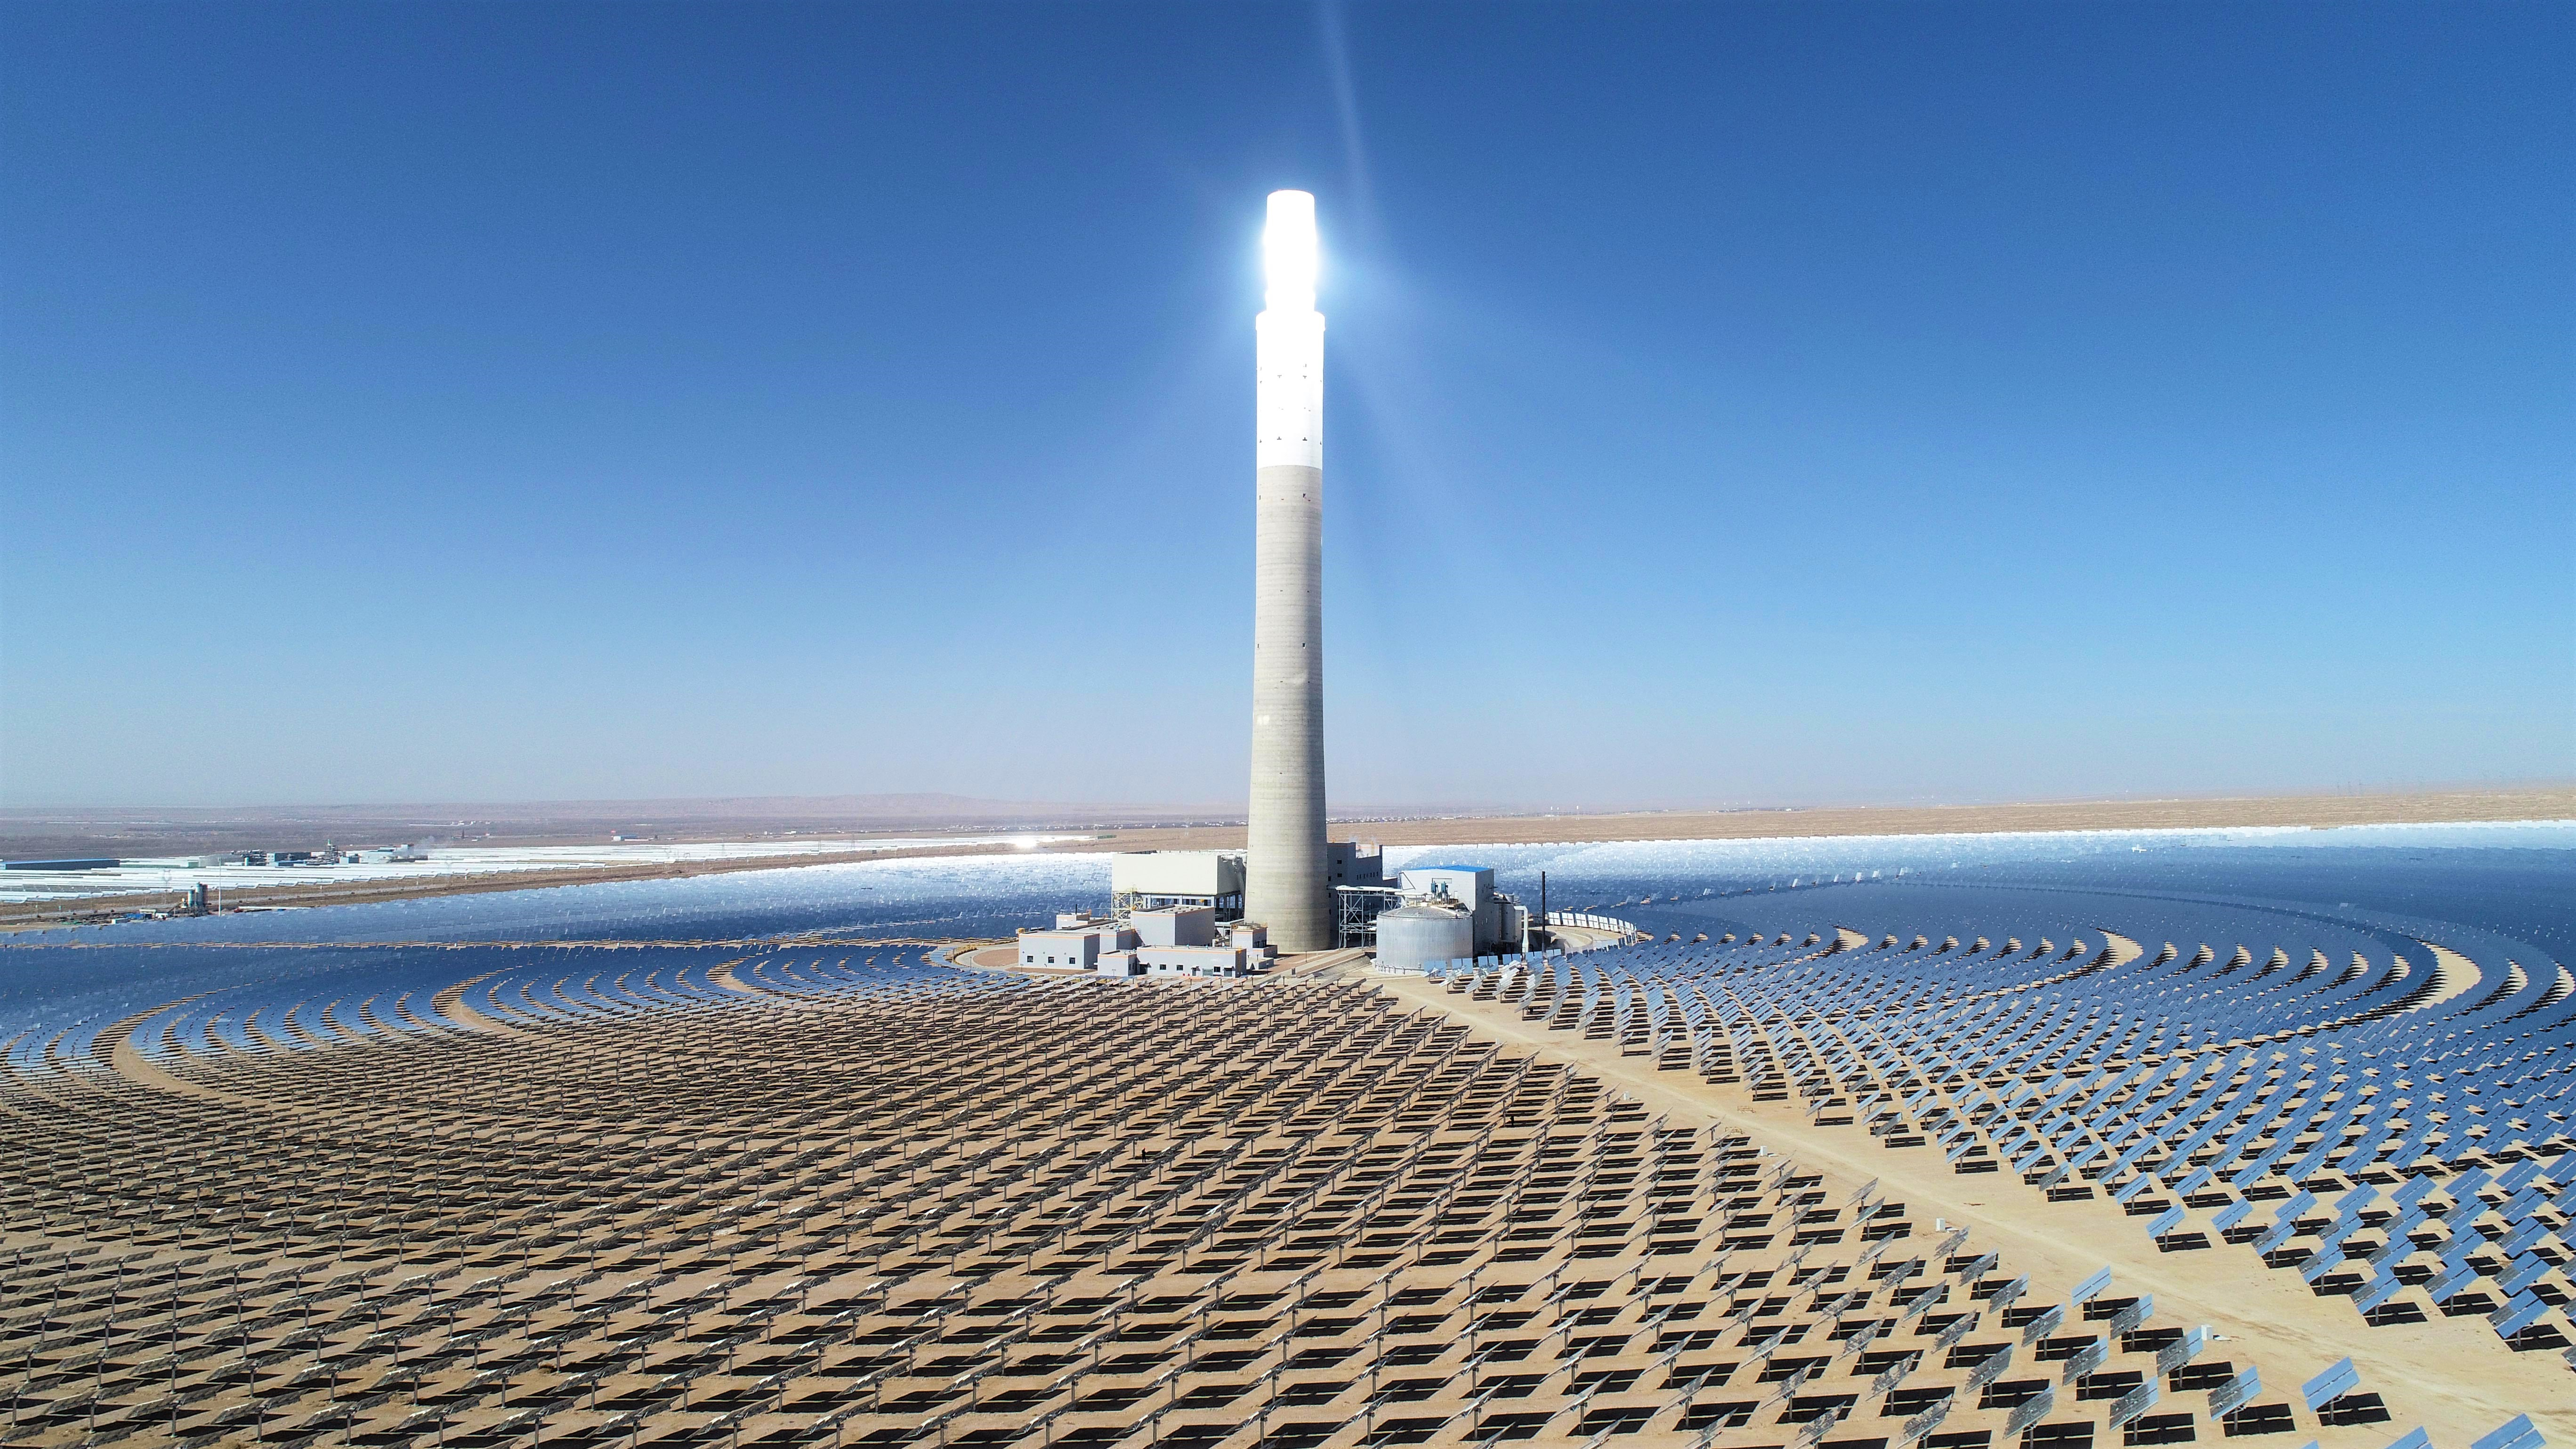
\includegraphics[scale = 0.07]{tower.jpg}
\caption{\kaishu 青海中控 {\rm 50mW + 10mW} 塔式光热电站}
\end{figure}
% TODO fig require
\subsection{问题重述}
塔式太阳能光热发电站由中心塔和其顶部的集热器和其周围的定日镜组成。定日镜水平转轴和纵向转轴能够控制俯仰角,两个转轴的交点是定日镜的镜面中点。定日镜的安装高度是镜面中点和地面的距离。定日镜的作用是将太阳光反射到中心塔的集热器。定日镜正常运作时,其能够将太阳中心发出的光线反射到集热器中心。

以中心为东经 \(98.5^\circ\),北纬 \(39.4 ^\circ\),海拔 \(3000\, \mathrm{m}\),半径 \(350 \, \mathrm{m}\)的区域内建设定日镜场。
\paragraph{问题1}
对于每一个定日镜设定镜面尺寸为 \(6 \,\mathrm{m} \times 6 \, \mathrm{m}\),安装高度为 \(4 \,\mathrm{m}\),在附件之中给出所有定日镜中心的位置,要求给出在此设置之下,建立定日镜镜场的数学模型,给出镜场的年平均光学效率、年平均输出热功率、单位镜面积年平均输出热功率。所得结果填入表格。
\paragraph{问题2}
现要求设计定日镜场的布局和参数,在定日镜场达到年平均输出热功率达到额定功率 \(60 \, \mathrm{MW}\)的条件下,确定以下5个参数:中心塔的位置坐标、定日镜的尺寸、安装高度、定日镜数目、定日镜位置,使得单位镜面面积年平均输出热功率尽量大。将结果填入表内,并将各参数按照指定格式保存在 \texttt{result2.xlsx}之中。
